\documentclass[conference]{IEEEtran}
\IEEEoverridecommandlockouts

\usepackage{cite}
\usepackage{amsmath,amssymb,amsfonts}
\usepackage{algorithmic}
\usepackage{graphicx}
\usepackage{textcomp}
\usepackage{xcolor}
\def\BibTeX{{\rm B\kern-.05em{\sc i\kern-.025em b}\kern-.08em
    T\kern-.1667em\lower.7ex\hbox{E}\kern-.125emX}}
\begin{document}

\title{Detecting Social Media Bots: Final Report}

\author{
\IEEEauthorblockN{Moaz Ali\textsuperscript{1}, Gabriel Alfredo Siguenza\textsuperscript{2}, Roberto Rafael Reyes\textsuperscript{3},\\ Stephanie Pocci\textsuperscript{4}, Prabhakara Kambhammettu\textsuperscript{5}, Alan Cortez\textsuperscript{6}
}
\IEEEauthorblockA{\textit{Department of Computer Science} \\
\textit{California State Polytechnic University, Pomona}\\
Pomona, USA \\}}

\maketitle

\begin{abstract}
Social media platforms are often targeted by automated accounts, known as bots, which can deceive public opinion, spread misinformation, and influence discourse through deceptive means. This project presents a data-driven approach to detecting bot accounts on VK.com, Russia's largest social network. Using a data set of more than 12,000 profiles and more than 60 features, we applied traditional classification techniques to determine whether accounts were likely operated by bots or humans. We implemented and compared Naive Bayes, Decision Tree, Logistic Regression, and Random Forest classifiers, highlighting the benefits of a structured and interpretable modeling pipeline.
\end{abstract}

\begin{IEEEkeywords}
Data Mining, Classification, Social Bots, VK.com, Pattern Detection
\end{IEEEkeywords}

\section{Introduction}
Automated accounts (bots) have become increasingly sophisticated, often mimicking human behavior to deceive users and manipulate information. Although most research has focused on English-speaking platforms like Twitter and Facebook, this project focuses on VK.com, where bot presence remains understudied yet impactful.

Detecting bots is a nontrivial problem because bots often use strategies to emulate legitimate behaviors, such as having profile pictures, posting regularly, or mimicking engagement patterns. This requires the use of structured, data-driven detection techniques.

Our team’s goal was to build a reliable bot classification model. We collaborated to pre-process the data, engineer features, train and evaluate multiple models, and thoroughly document the results. Each step in the pipeline was discussed and improved iteratively on the basis of initial findings and feedback.

\section{Dataset}
The data set used for this study is publicly available on Kaggle\cite{b1}. It contains labeled information for VK.com accounts, specifically labeled as bots or human users. The key characteristics include:

\begin{itemize}
    \item 12,000+ instances.
    \item 60+ features, both numeric and categorical.
    \item Label column (`target`), with 0 representing humans and 1 for bots.
\end{itemize}

\subsection{Features Overview}
Some notable feature groups:
\begin{itemize}
    \item \textbf{Account Attributes:} has\_domain, has\_photo, gender, is\_verified.
    \item \textbf{Activity Metrics:} posts\_count, reposts\_ratio, likes\_average.
    \item \textbf{Content Info:} text length, number of hashtags, uniqueness of text.
    \item \textbf{Engagement Patterns:} comments, views, post frequency.
\end{itemize}

\subsection{Target Class}
The `target` feature is the binary class label used for classification. It was evenly distributed between classes, simplifying model evaluation and mitigating bias.

\section{Methodology}
\subsection{Preprocessing}
We addressed several data quality issues:
\begin{itemize}
    \item \textbf{Missing Values:} All "Unknown" values and blanks were converted to NaN.
    \item \textbf{Imputation:} For numeric columns, median was used; for categorical, mode was applied.
    \item \textbf{Normalization:} Applied Min-Max scaling to all numeric columns to bring them into a range of 0-1.
    \item \textbf{Encoding:} Used one-hot encoding on categorical features to convert them into a machine-readable format.
\end{itemize}

\subsection{Train/Test Split}
To ensure fairness, we split the dataset using stratified sampling:
\begin{itemize}
    \item 80\% of the data used for training.
    \item 20\% used for testing.
    \item The `stratify` parameter ensured class balance in both sets.
\end{itemize}

\subsection{Model Training}
We implemented the following classifiers:
\begin{enumerate}
    \item \textbf{Naive Bayes:} A probabilistic model good for baseline comparisons.
    \item \textbf{Decision Tree:} Captures simple rule-based patterns.
    \item \textbf{Logistic Regression:} An effective linear model often used in binary classification.
    \item \textbf{Random Forest:} Ensemble model combining multiple decision trees, providing high accuracy and robustness.
\end{enumerate}

Each model was trained on the cleaned data, then serialized using \texttt{joblib} for testing and reuse.

\subsection{Evaluation}
We tested each model on the hold-out test set using:
\begin{itemize}
    \item Accuracy
    \item Precision
    \item Recall
    \item F1 Score
    \item Confusion Matrix
\end{itemize}

\section{Results}

\subsection{Evaluation Metrics}
% Your model performance descriptions...

% INSERT FIGURES HERE
\begin{figure}[htbp]
\centerline{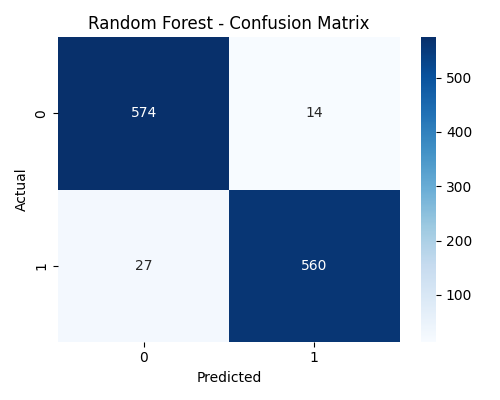
\includegraphics[width=\linewidth]{RF_CM.png}}
\caption{Confusion Matrix for the Random Forest model. It achieved high accuracy with minimal false positives and false negatives.}
\label{fig:rf_cm}
\end{figure}

\begin{figure}[htbp]
\centerline{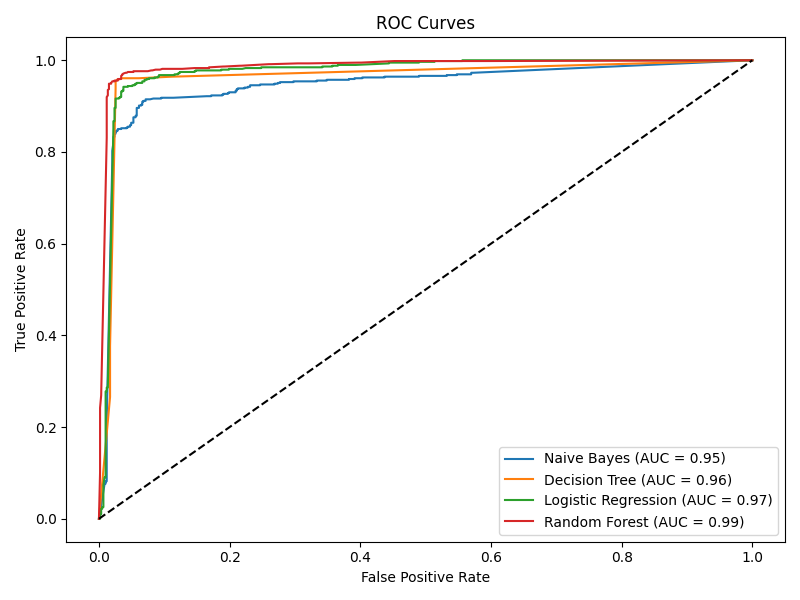
\includegraphics[width=\linewidth]{ROC_Curve.png}}
\caption{ROC Curve for all classifiers. Random Forest achieved the highest AUC (0.99), indicating excellent discriminatory power.}
\label{fig:roc_curve}
\end{figure}

\begin{figure}[htbp]
\centerline{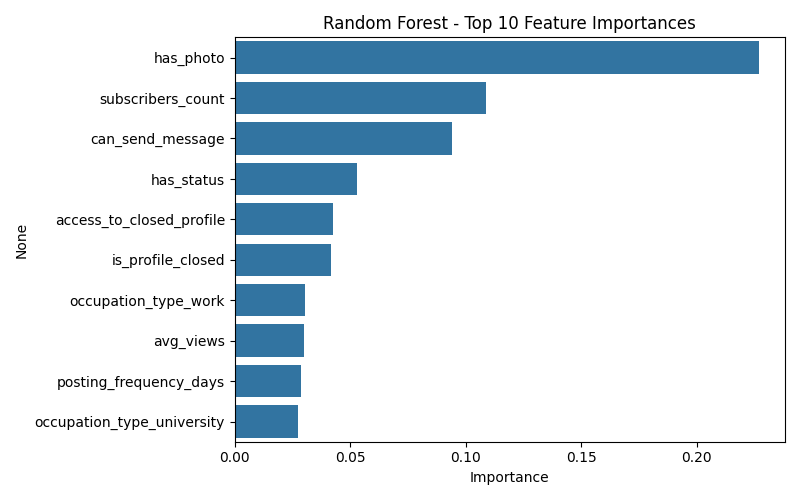
\includegraphics[width=\linewidth]{Random_Forest_Top_Features.png}}
\caption{Top features used by the Random Forest model. These contributed the most to the classification task.}
\label{fig:rf_features}
\end{figure}

\begin{figure}[htbp]
\centerline{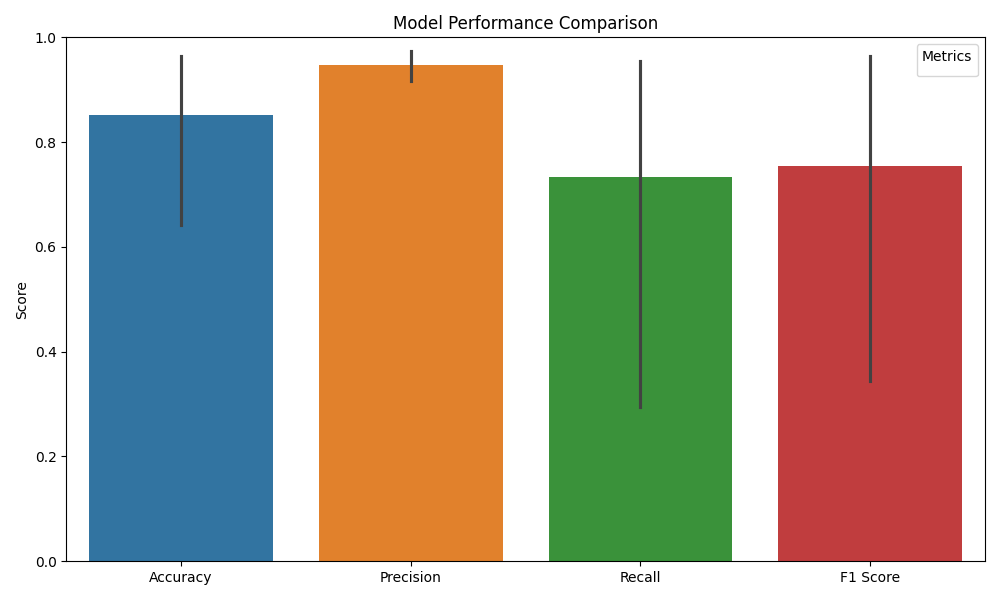
\includegraphics[width=\linewidth]{models_average.png}}
\caption{Average performance of all models across accuracy, precision, recall, and F1-score. Random Forest and Decision Tree stand out.}
\label{fig:models_avg}
\end{figure}

% Analysis and commentary


\subsection{Discussion}
The Random Forest classifier outperformed others, likely due to its ability to capture complex interactions among features. While Logistic Regression performed well, it lacked the flexibility to capture nonlinear patterns. Naive Bayes performed poorly on correlated features.

\section{Related Work}

Bot detection has been extensively researched across various social media platforms, particularly Twitter, which has been a primary focus due to its open API and high bot activity. Tools like Botometer (formerly BotOrNot) have emerged as prominent frameworks, leveraging a wide range of features including content-based (e.g., tweet frequency, sentiment analysis), temporal (e.g., posting patterns), and network-based features (e.g., retweet/follower networks). These methods have proven effective in identifying simple and sophisticated bots but often require large-scale data collection and computational resources.

Recent studies have also explored machine learning and deep learning approaches to enhance detection performance. Some employ recurrent neural networks (RNNs) or graph neural networks (GNNs) to capture temporal and structural information. Others use unsupervised techniques like clustering or anomaly detection to flag unusual account behaviors.

However, these methods typically depend on a combination of user content, social graphs, and interaction patterns, which may not always be accessible due to API limitations or privacy concerns. Moreover, the high dimensionality and heterogeneity of such data increase computational complexity, making real-time or large-scale detection challenging.

In contrast, our project focuses solely on profile-level features, such as account creation date, number of followers, profile completeness, and activity metadata. This lightweight approach demonstrates that effective bot detection can still be achieved without relying on content or network-level information. Similar minimalist approaches have been less explored but show promise in scenarios with limited access to full user activity data. Our work contributes to this growing area by applying it to VK.com, a relatively underexplored platform in bot detection literature, and achieving competitive classification performance with significantly reduced overhead.


Other research has focused on advanced pattern recognition and graph-based user modeling to identify coordinated or anomalous behavior. While these methods may offer improvements, they often require more data and processing power.

\section{Conclusion}

In this study, we developed a structured classification pipeline for detecting social media bots on VK.com using fundamental data mining techniques. By relying solely on profile-level features—such as friend counts, activity ratios, and account metadata—we demonstrated that even simple attributes, when properly prepared and engineered, can lead to effective classification performance. Our approach leveraged ensemble learning methods, which improved robustness and accuracy while maintaining computational efficiency.

A key takeaway from our work is the significant impact of thorough data preprocessing and systematic model evaluation. Despite the simplicity of our feature set, careful attention to handling missing values, feature scaling, and class balancing contributed to the overall success of the pipeline. These findings support the notion that strong baseline models can be built without complex feature sets or deep architectures, especially in settings with limited data access.

Looking ahead, there are several promising directions for future work:

\begin{itemize} \item \textbf{Feature Selection and Dimensionality Reduction:} Applying techniques such as Recursive Feature Elimination (RFE), PCA, or mutual information analysis could enhance model interpretability and performance. \item \textbf{Integration of Text-Based and Graph Data:} Including content-level features (e.g., post frequency, language use) and network structure (e.g., follower/friend graphs) could offer richer context and improve detection of more sophisticated bots. \item \textbf{Real-Time Detection Systems:} Developing a live system capable of continuously monitoring VK activity and flagging suspicious accounts in real-time would significantly increase the practical utility of this work. \end{itemize}

Ultimately, our work provides a strong foundation for further research into lightweight yet effective bot detection methods, especially on platforms like VK.com, where traditional detection frameworks are less established.


For future work, we plan to explore:
\begin{itemize}
    \item Feature selection and dimensionality reduction.
    \item Integration of text-based and social graph data.
    \item Real-time detection systems for live VK data.
\end{itemize}

\section{References}
\begin{thebibliography}{00}
\bibitem{b1} Users vs Bots Classification Dataset, Kaggle. https://www.kaggle.com/datasets/juice0lover/users-vs-bots-classification
\bibitem{b2} Tan, Pang-Ning, et al. Introduction to Data Mining. Pearson, 2018.
\bibitem{b3} Scikit-learn: Machine Learning in Python. https://scikit-learn.org
\bibitem{b4} Davis, C.A., Varol, O., Ferrara, E., Flammini, A., Menczer, F. (2016). BotOrNot: A system to evaluate social bots. WWW '16 Companion.
\end{thebibliography}

\section{Links to Files}
\begin{itemize}
    \item 
\end{itemize}

\end{document}
